\chapter{Statistical analysis}
\label{ch:stat-ana}

\par Statistical analysis is a process to analyze collision data in the signal and control regions with statistical models to test physics hypothesis. 
In new physics search analysis, one can do hypothesis testing on new physics if relatively obvious excesses are observed in data versus Monte-Carlo background comparison plots. 
In this analysis, since the no obvious excesses happen, model exclusion becomes a meaningful target to achieve. 
New physics model exclusion with collision data can be turned viewed as parameters confidential interval estimation. 
In particle physics, the CLs method\cite{Read:2002hq} is a powerful and proven method for model parameters limit setting. 
In this chapter, the CLs strategies for this analysis are described in Section~\ref{sec:cls}, and then, the fit results are demonstrated in Section~\ref{sec:limitres}. 

\section{CLs method}
\label{sec:cls}

\par The aim of statistical analysis is to evaluate the upper limit of new physics model parameters , for example, mass of z prime in 2HDM model, given observation and nuisance parameters. 
Confidence interval is associated with a confidence level that the true parameter is in the proposed range. 
The CLs method, which is a statistical estimation to evaluate confidence interval of parameters of a model with data, is the approach that used to set the upper limit of new physics model parameters in this analysis.

\par The CLs method is not the only approach to set the upper limit of model parameters. 
One can also use the traditional frequentist approach or novel Bayesian way instead. 
The Bayesian way is not preferred by experimental physicists because it needs to set a prior on the new physics model itself.
The traditional frequentist approach has trouble when the signal is too small. 
It will give a negative upper limit since it estimates data yield with confidence level, then subtract background yield.
Therefore, the CLs method, as a modified frequentist approach, is introduced with a normalization on background only probability to avoid this issue.

\par Like all other upper limit estimation approaches, one needs to build likelihood function first, count data and background yields in different event categories, and deal with the nuisance parameters to get limit setting result. 
More details will be covered in the rest of this section.

\subsection{Likelihood definition}

\par The likelihood function is a reflection of probability of event yields in signal region. 
It is obvious that the event count in the signal region follows Poisson distribution, since each event have a finite probability to be observed in the signal region.
Therefore, the statistical analysis of the data uses a binned likelihood function constructed as the product of Poisson probability terms,
\begin{equation}
\mathrm{Poisson}\,(n|\mu S+B)\left[ \prod_{b\in \text{bins}}^{n} \frac{\mu \nu^{\mathrm{sig}}_{b}+\nu^{\mathrm{bkg}}_{b}}{\mu S+B} \right],
\end{equation}
where $\mu$, a signal strength parameter, multiplies the expected signal yield $\nu^{\mathrm{sig}}_b$ in each histogram bin $b$, and $\nu^{\mathrm{bkg}}_b$ represents the background content for bin $b$. 
The dependence of the signal and background predictions on the systematic uncertainties is described by a set of nuisance parameters (NP) $\theta$, which are parameterized by Gaussian or log-normal priors. 
The latter are used for normalization uncertainties in order to maintain a positive likelihood.

\par This profile of likelihood, together with Monte-Carlo simulation of signal and background, are used to model the data yields.

\subsection{Nuisance parameters}

\par In statistics, nuisance parameters are the parameters which are not of immediate interest but which must be accounted for in the analysis of those parameters which are of interest. 
Two types of nuisance parameters are considered in this analysis:
\begin{itemize}
    \item \textbf{Normalization related nuisance parameters}: These nuisance parameters are single number correction that comes from cross-section calculation, Monte-Carlo template and relative acceptance, etc.. 
    A full list of normalization of this type nuisance parameters are shown in Table~\ref{tab:np-norm1} and~\ref{tab:np-norm2}.
    \item \textbf{Shape related nuisance parameters}: These nuisance parameters are introduced by either detector or theory, and will be used to fit observables. 
    A full list of normalization of this type nuisance parameters are shown in Table~\ref{tab:np-shape1} and~\ref{tab:np-shape2}.
\end{itemize}

\begin{table}[ht]
    \centering
    \scriptsize
    \begin{tabular}{|p{2.5cm}|p{1.5cm}|p{3cm}|p{2.5cm}|p{1.5cm}|}
        \hline
        NP Name & Prior & Description & Applied to sample & Applied in region \\
        \hline
        \texttt{norm\_Zhf} & flat & normalisation of Zhf template & Zhf & all \\
        \texttt{norm\_Whf} & flat & normalisation of Whf template & Zhf & all \\
        \texttt{norm\_ttbar} & flat & normalisation of $t\bar{t}$ template & $t\bar{t}$ & all \\
        \hline
        \hline
        \texttt{stopsNorm} & 3.7\% & single top $s$-channel inclusive normalisation & $s$-channel s.top & all \\
        \texttt{stoptNorm} & 3.9\% & single top $t$-channel inclusive normalisation & $t$-channel s.top & all \\
        \texttt{stopWtNorm} & 5.4\% & single top $Wt$-channel inclusive normalisation & $Wt$-channel s.top & all \\
        \texttt{WWNorm} & 25\% & inclusive normalisation of $WW$ & WW & all \\
        \texttt{WZNorm} & 26\% & inclusive normalisation of $WZ$ & WZ & all \\
        \texttt{ZZNorm} & 20\% & inclusive normalisation of $ZZ$ & ZZ & all \\
        \texttt{HiggsNorm} & 22\% & inclusive normalisation of SM $Vh(b\bar{b})$ & VHbb & all \\
        \hline
        \hline
        \texttt{ZcllNorm} & 30\% & inclusive normalisation uncertainty for $Zcl$ & Zcl & all \\
        \texttt{WcllNorm} & 30\% & inclusive normalisation uncertainty for $Wcl$ & Zcl & all \\
        \texttt{ZlNorm} & 10\% & inclusive normalisation uncertainty for $Zl$ & Zl & all \\
        \texttt{WlNorm} & 10\% & inclusive normalisation uncertainty for $Wl$ & Wl & all \\
        \hline
        \hline
        \texttt{ZhfNorm\_L0} & 20\% & relative acceptance difference of Zhf between 0 and 2L regions & Zhf & 0L \\
        \texttt{WhfNorm\_L0} & 20\% & relative acceptance difference of Zhf between 0 and 2L regions & Whf & 0L \\
        \hline
    \end{tabular}
    \caption{Nuisance parameters associated to theoretical uncertainties that affect the normalisation/relative acceptance with their prior uncertainties (in the case of Gaussian priors the numbers correspond to the $1\sigma$ prefit uncertainties).}
    \label{tab:np-norm1}
\end{table}

\begin{table}[ht]
    \centering
    \scriptsize
    \begin{tabular}{|p{2.5cm}|p{1.5cm}|p{3cm}|p{2.5cm}|p{1.5cm}|}
        \hline
        NP Name & Prior & Description & Applied to sample & Applied in region \\
        \hline
        \texttt{WblWhfRatio} & 20\% & uncertainty on $\sigma(Wbl)$/$\sigma(Whf)$ & Wbl & 0L, 1L \\
        \texttt{WccWhfRatio} & 20\% & uncertainty on $\sigma(Wcc)$/$\sigma(Whf)$ & Wcc & 0L, 1L \\
        \texttt{WbcWhfRatio} & 20\% & uncertainty on $\sigma(Wbc)$/$\sigma(Whf)$ & Wbc & 0L, 1L \\
        \texttt{ZblZhfRatio} & 20\% & uncertainty on $\sigma(Zbl)$/$\sigma(Zhf)$ & Zbl & all \\
        \texttt{ZccZhfRatio} & 20\% & uncertainty on $\sigma(Zcc)$/$\sigma(Zhf)$ & Zcc & all \\
        \texttt{ZbcZhfRatio} & 20\% & uncertainty on $\sigma(Zbc)$/$\sigma(Zhf)$ & Zbc & all \\
        \hline
        \hline
        \texttt{SysTopMETshape} & 20\% & relative acceptance difference across \met bins & $t\bar{t}$ & all except lowest \met bin \\
        \texttt{SysWhfMETshape} & 20\% & relative acceptance difference across \met bins & Whf & all except lowest \met bin \\
        \texttt{SysZhfMETshape} & 20\% & relative acceptance difference across \met bins & Zhf & all except lowest \met bin \\
        \hline
        \hline
        \texttt{ATLAS\_LUMI} & 1.7\% & luminosity uncertainty & all & all \\
        \hline
    \end{tabular}
    \caption{Nuisance parameters associated to theoretical uncertainties that affect the normalisation or relative acceptance with their prior uncertainties (in the case of Gaussian priors the numbers correspond to the $1\sigma$ prefit uncertainties).}
    \label{tab:np-norm2}
\end{table}

\begin{table}[ht]
    \centering
    \scriptsize
    \begin{tabular}{|p{3.5cm}|p{2.5cm}|p{1.5cm}|p{2cm}|p{1.5cm}|}
        \hline
        NP Name & Description & Treatment & Applied to sample & Applied in region \\
        \hline
        \texttt{SysttbarMbb} & Sec.~\ref{sec:thy-sys-unc} & - & $t\bar{t}$ & all \\
        \texttt{SysttbarMbb} & Sec.~\ref{sec:thy-sys-unc} & - & single-top $Wt$ & all \\
        \texttt{SysWMbb} & Sec.~\ref{sec:thy-sys-unc} & - & Whf, Wcl, Wl & all \\
        \texttt{SysZMbb} & Sec.~\ref{sec:thy-sys-unc} & - & Zhf, Zcl, Zl & all \\
        \texttt{SysWWMbb} & Sec.~\ref{sec:thy-sys-unc} & - & WW & all \\
        \texttt{SysWZMbb} & Sec.~\ref{sec:thy-sys-unc} & - & WZ & all \\
        \texttt{SysZZMbb} & Sec.~\ref{sec:thy-sys-unc} & - & ZZ & all \\
        \hline
    \end{tabular}
    \caption{Nuisance parameters associated to theoretical uncertainties that affect the $m(b\bar{b})$ shape and their treatment (S=smoothed, Sym1=symmetrised (one-sided systematic), Sym2=symmetrised (two-sided systematic)).}
    \label{tab:np-shape1}
\end{table}

\begin{table}[ht]
    \centering
    \scriptsize
    \begin{tabular}{|p{3.5cm}|p{2.0cm}|p{1.5cm}|p{2cm}|p{1.5cm}|}
        \hline
        NP Name & Description & Treatment & Applied to sample & Applied in region \\
        \hline
        \texttt{EL\_EFF\_*} & Sec.~\ref{sec:exp-sys-unc} & - & all & all \\
        \texttt{EG\_RESOLUTION\_*} & Sec.~\ref{sec:exp-sys-unc} & S & all & all \\
        \texttt{EG\_SCALE\_*} & Sec.~\ref{sec:exp-sys-unc} & S & all & all \\
        \texttt{MUON\_EFF\_*} & Sec.~\ref{sec:exp-sys-unc} & - & all & all \\
        \texttt{MUON\_SAGITTA\_*} & Sec.~\ref{sec:exp-sys-unc} & - & all & all \\
        \texttt{MUON\_SCALE\_*} & Sec.~\ref{sec:exp-sys-unc} & S & all & all \\
        \texttt{MUON\_MS\_*} & Sec.~\ref{sec:exp-sys-unc} & S & all & all \\
        \texttt{MUON\_ID\_*} & Sec.~\ref{sec:exp-sys-unc} & S & all & all \\
        \texttt{TAUS\_TRUEELECTRON\_*} & Sec.~\ref{sec:exp-sys-unc} & - & all & all \\
        \texttt{TAUS\_TRUEHADTAU\_EFF\_*} & Sec.~\ref{sec:exp-sys-unc} & - & all & all \\
        \texttt{TAUS\_TRUEHADTAU\_SME\_*} & Sec.~\ref{sec:exp-sys-unc} & S & all & all \\
        \texttt{JET\_EffectiveNP\_*} & Sec.~\ref{sec:exp-sys-unc} & S, Sym2 & all & all \\
        \texttt{JET\_Eta*} & Sec.~\ref{sec:exp-sys-unc} & S, Sym2 & all & all \\
        \texttt{JET\_JET\_Flavor\_*} & Sec.~\ref{sec:exp-sys-unc} & S, Sym2 & all & all \\
        \texttt{JET\_CombMass\_*} & Sec.~\ref{sec:exp-sys-unc} & S, Sym2 & all & all \\
        \texttt{JET\_JET\_LargeR\_*} & Sec.~\ref{sec:exp-sys-unc} & S, Sym2 & all & all \\
        \texttt{JET\_JET\_MassRes\_*} & Sec.~\ref{sec:exp-sys-unc} & S, Sym2 & all & all \\
        \texttt{JET\_Pileup\_*} & Sec.~\ref{sec:exp-sys-unc} & S, Sym2 & all & all \\
        \texttt{JET\_PunchThrough} & Sec.~\ref{sec:exp-sys-unc} & S, Sym2 & all & all \\
        \texttt{JET\_RelativeNonClosure} & Sec.~\ref{sec:exp-sys-unc} & S, Sym2 & all & all \\
        \texttt{JET\_BJES\_Response} & Sec.~\ref{sec:exp-sys-unc} & S, Sym2 & all & all \\
        \texttt{JET\_JVT\_*} & Sec.~\ref{sec:exp-sys-unc} & S, Sym2 & all & all \\
        \texttt{JET\_fJVT\_*} & Sec.~\ref{sec:exp-sys-unc} & S, Sym2 & all & all \\
        \texttt{JET\_SingleParticle} & Sec.~\ref{sec:exp-sys-unc} & S, Sym2 & all & all \\
        \texttt{JET\_JER\_*} & Sec.~\ref{sec:exp-sys-unc} & S, Sym1 & all & all \\
        \texttt{FT\_EFF\_*} & Sec.~\ref{sec:exp-sys-unc} & S, Sym2 & all & all \\
        \texttt{METTrig\_*} & Sec.~\ref{sec:exp-sys-unc} & S & all & all \\
        \texttt{MET\_SoftTrk\_Scale\_*} & Sec.~\ref{sec:exp-sys-unc} & S & all & all \\
        \texttt{MET\_SoftTrk\_Reso\_*} & Sec.~\ref{sec:exp-sys-unc} & S, Sym1 & all & all \\
        \texttt{PRW\_DATASF} & Sec.~\ref{sec:exp-sys-unc} & - & all & all \\
        \hline
    \end{tabular}
    \caption{Nuisance parameters associated to detector systematics (affecting both shape and normalisation) and their treatment (S=smoothed, Sym1=symmetrised (one-sided systematic), Sym2=symmetrised (two-sided systematic)).}
    \label{tab:np-shape2}
\end{table}  

\par All nuisance parameters mentioned above will be integrated together with likelihood function to set upper limit using CLs method.

\section{Limit setting result}
\label{sec:limitres}

\par After the CLs strategy is well set up in the previous section, the Z'-2HDM model can be constrained by the observed data. 
There are two interesting parameters in this new physics model: mass of Z' and mass of A as dark matter candidate. 
Limit setting on signal strength is implemented on a two dimensional scan on these two parameters.

\par A result of limit setting on signal strength is shown in the Fig~\ref{fig:zprime-2hdm-limit}. 
It indicates that the mass of Z' can be excluded up to 2900 GeV in expected exclusion, 2700 GeV in observed exclusion respectively, while the mass of A is excluded to 700 GeV in expected exclusion, while 650 GeV in observed exclusion.

\begin{figure}[!htb]
    \centering
    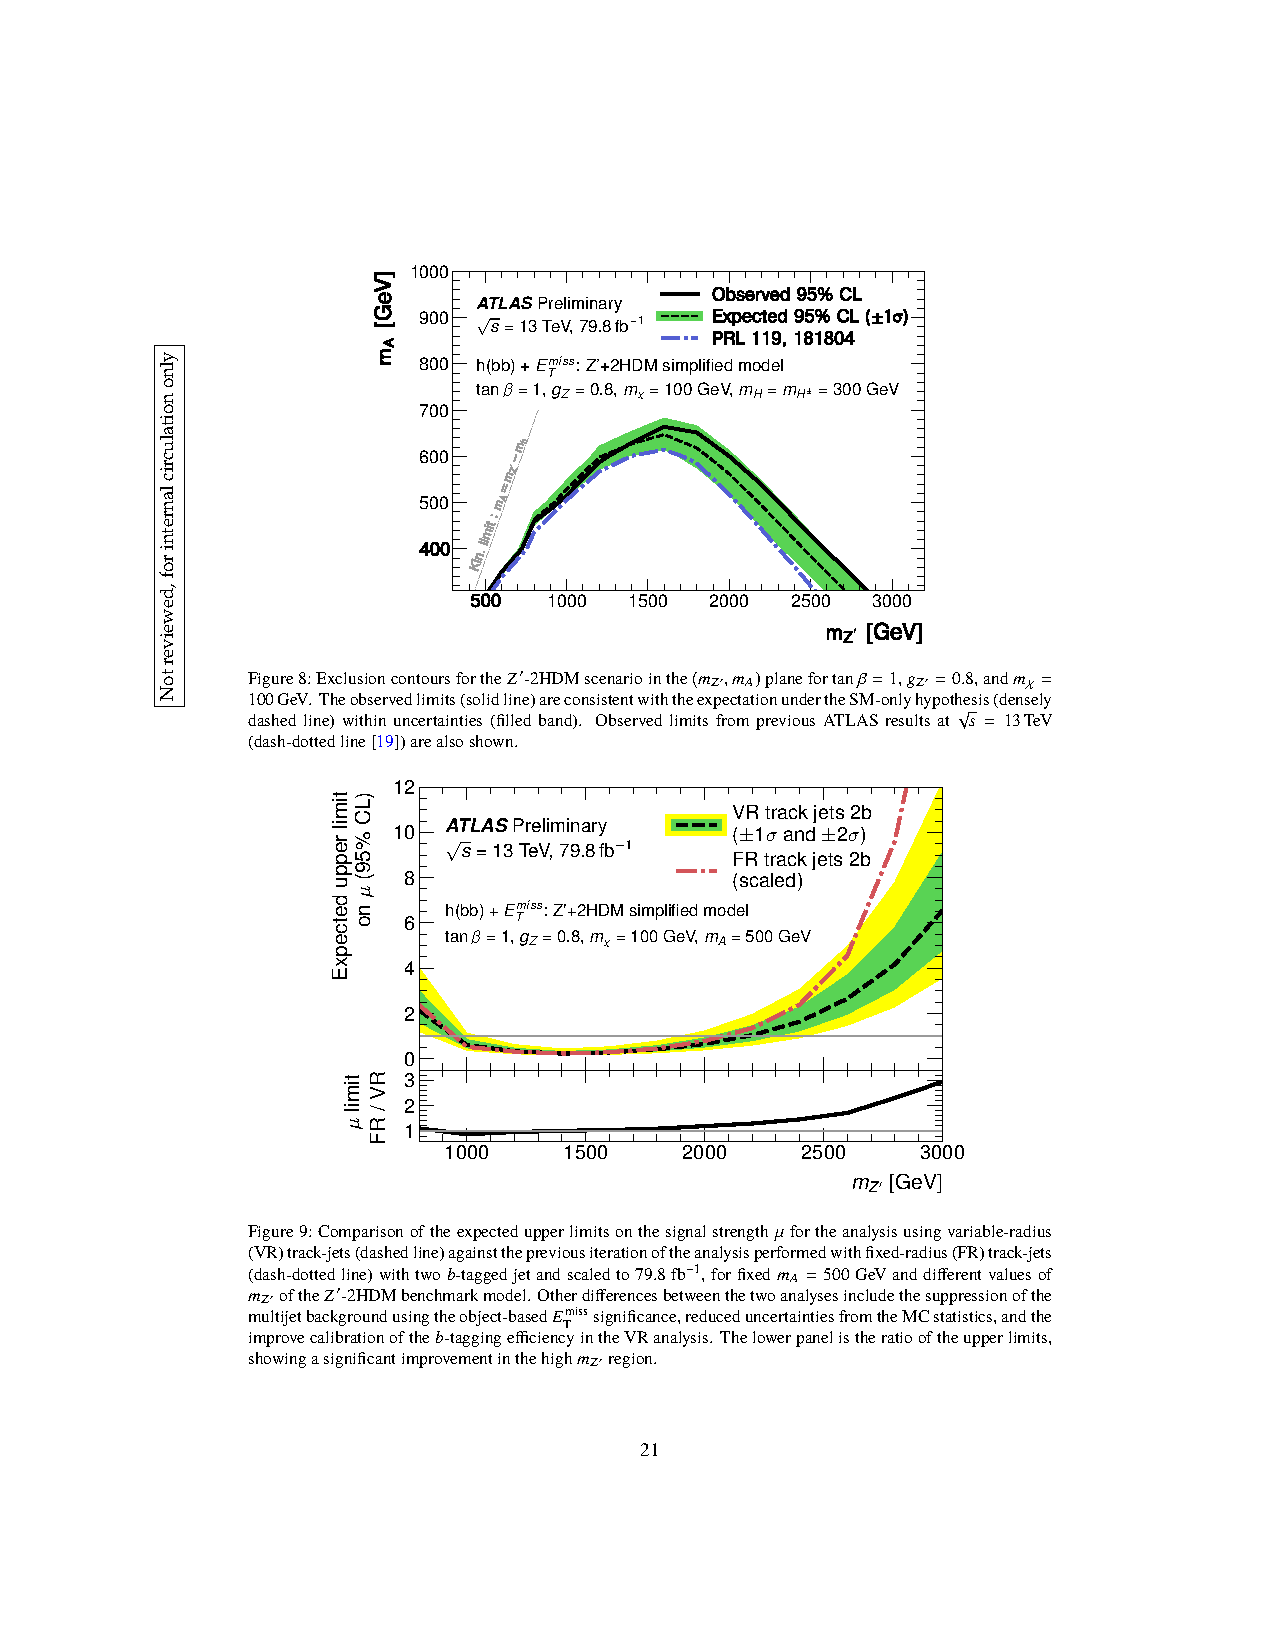
\includegraphics[width=12cm, height=9cm, trim={2.5cm 7.5cm 17.6cm 8cm}, clip]{chapters/c9/figures/ZPrime2HDMLimit.pdf}
    \caption{Fractional uncertainty on $\mu$ due to data statistics for each Z'-2HDM signal point.}
    \label{fig:zprime-2hdm-limit}
\end{figure}
